\section[Introducción]{Introducción}
\subsection[Contexto]{Contexto}
\begin{frame}
    \frametitle{Contexto}
    \begin{columns}
      \column{0.6\textwidth}
    \begin{enumerate}
      \item \textbf{La información visual} es cada vez más \textbf{importante}.
        \begin{itemize}
          \item Tanto para el entretenimiento como para el ámbito biomédico.
        \end{itemize}
      \item{Tarea de medir y cuantificar} la calidad perceptual humana de una imagen (IQA). 
        \begin{itemize}
          \item Factores importantes: \textbf{contenido, contraste, distorsiones y la percepción humana}
        \end{itemize}
    \end{enumerate}
    \column{0.4\textwidth}
    \begin{figure}
      \begin{center}
        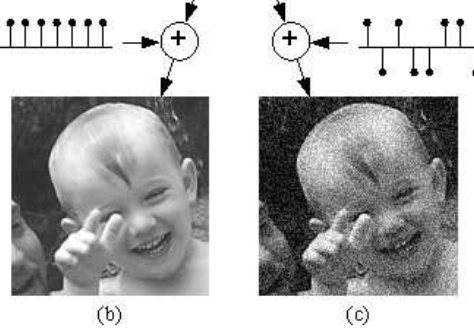
\includegraphics[width=\textwidth]{imagenes/chapter1/failure_minkowski_metricBIG}
      \end{center}
      \caption{Imágenes distorsionadas equidistantes\footnotemark}
    \end{figure}
  \end{columns}
  \vspace{-.2cm}
  \footcitetext{MinkowskiFailure}
\end{frame}

\note{
  Para empezar, hay que tenerse en cuenta que existe 
una demanda incremental de aplicaciones, tanto para el entretenimiento 
como para el estudio biomédico. Donde la información visual cada vez tiene un rol 
más importante. Sin embargo, la calidad de dicha información puede 
verse mermada con las etapas de adquisición, procesado, transmisión 
y reproducción.
Es por ello que poder evaluar dicha calidad se ha vuelto un 
tema cada vez más importante.
Para resolver este problema es necesario tener en cuenta diversos factores como 
el contenido de la imagen, nivel de contraste, posibles distorsiones y, por supuesto,
conocimientos del sistema visual humano. 
Por ello mismo presenta un alta complejidad.
Por ejemplo, una aproximación sencilla sería optar por métodos de sensibilidad 
al error o distancias. 
No obstante, eso es imponer un conjunto de suposiciones cuestionables. 
La más importante de ellas es que unifica la importancia de los factores 
mencionados anteriomente. 
Lamentable, eso no se cumple, como podemos observar en la imagen a la derecha.
En ella, dos pares de imágenes (b) y (c), generadas al sumar la misma constante 
pero permutando signo, presentan distinto nivel de agrado visual y aún así 
se clasifican como iguales.
}

\begin{frame}
  \frametitle{Subproblemas}
  \vspace{-.5cm}
  \begin{figure}
    \caption{Figuras (a) y (b): problemas con referencia (FR) y sin referencia (NR).}
    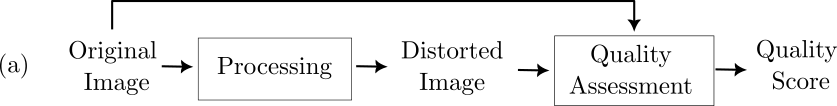
\includegraphics[width=0.8\textwidth]{imagenes/chapter1/HFullReferenceInk.png}
  \end{figure}
  \begin{figure}
    
\includegraphics[width=0.8\textwidth]{imagenes/chapter1/NoReferenceInk.png}
  \end{figure}
  \begin{enumerate}
    \item (b) es el subproblema más \textbf{difícil}.
    \item Debemos disponer de conocimientos generales sobre: 
      \begin{enumerate}
        \item Naturaleza de las imágenes.
        \item Efecto de las distorsiones.
      \end{enumerate}
  \end{enumerate}
\end{frame}

\note{
  Existen tres subproblemas presenten en el ámbito de IQA. 
Dos de ellos serían similar al ejemplo anterior. 
Donde tenemos acceso a la imagen original, o ciertas propiedades suyas, 
y podemos aplicar métodos basados en diferencia de características.
Se denominan con referencia o con referencia reducida si disponemos de información 
parcial.

No obstante, en el caso de la medicina no disponemos de dicha información de referencia. 
Es por ello que nos centraremos en el último subproblema, considerado el más 
difícil del campo.
Este sería la imagen (b), estimación sin referencia.
Para resolver este tipo de problemas, debemos disponer de conocimientos de la 
naturaleza de las imágenes y los efectos de las 
distorsiones sobre ellas. 
Lo que se denomina estadísticas de escena naturales. 
Veremos más ejemplos en adelante.

Primeramente, me gustaría hablar de las aplicaciones.
}


\subsection{Motivación}
\begin{frame}
  \frametitle{Aplicaciones}
  \begin{columns}
    \column{0.5\textwidth}
  \begin{enumerate}
      \item\textbf{Comparativa} entre algoritmos de compresión.
      \item\textbf{Recuperación} de la información.
      \item\textbf{Evaluar} errores de transmisión.
  \end{enumerate}
  \column{0.5\textwidth}
  \begin{figure}
    \begin{center}
      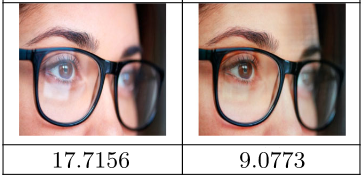
\includegraphics[width=0.85\textwidth]{imagenes/chapter1/Brisque}
    \end{center}
    \caption{
      Eliminación de reflejos en imágenes\footnote[frame]{\cite{BRISQUEExample}}
      con medida de calidad BRISQUE\footnote[frame]{\cite{BRISQUE}} (menor es mejor).
  }
  \end{figure}
  \end{columns}
\end{frame}

\note{
De ellas, destacan:
\begin{itemize}
\item Comparación de algoritmos de compresión, estimando la pérdida de información que producen.
 
\item Generación de mapas de calidad para el estudio de métodos de recuperación de 
información. Un ejemplo sería la imagen de la derecha donde se eliminan reflejos 
gracias una famosa medida de calidad 2D, BRISQUE.

\item Por último, este campo nos permite determinar la calidad de los servicios de transmisión y
entre otros.
\end{itemize}
}

\begin{frame}
  \frametitle{Motivación}
  \begin{columns}
    \column{0.5\textwidth}
    \begin{enumerate}
    \item Cada vez \textbf{más frecuentemente} se emplean volúmenes tridimensionales.
    \item Las contribuciones relativas al IQA en la medicina resulta en: 
      \begin{itemize}
        \item \textbf{Reducción de costes}. 
        \item Reducción de tiempo de consulta.
        \item \textbf{Mejora de calidad del diagnóstico}.
      \end{itemize}
    \item La naturaleza de las imaǵenes médicas \textbf{reduce} la precisión de modelos IQA estándares.
    \end{enumerate}
  \column{0.5\textwidth}
  \begin{figure}
    \begin{center}
      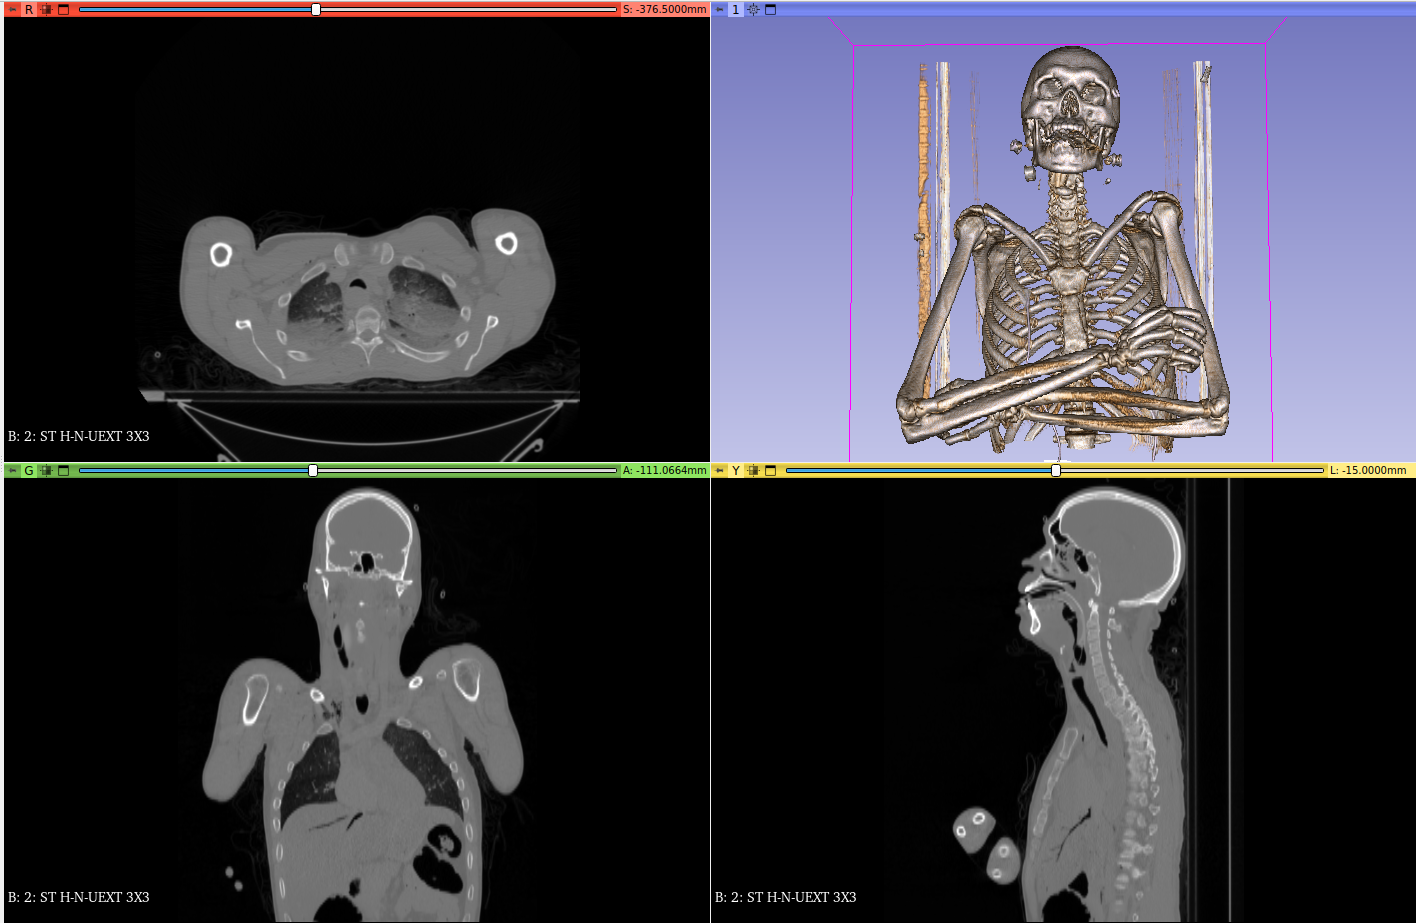
\includegraphics[width=0.95\textwidth]{imagenes/chapter1/SlicerVisualization}
    \end{center}
    \caption{Ejemplo de visualización 3D (Slicer\footnotemark).}
  \end{figure}
  \end{columns}
  \footcitetext{Slicer3D}
\end{frame}

\note{
Nuestra motivación viene dos grandes razones. 
La primera es que cada vez más frecuentemente se emplean volúmenes 3D, 
como tomografías computarizadas o
resonancias magnéticas en lugar de radiografías convencionales. 
Esto es porque proporcionan una visión más completa y detallada de la anatomía 
y las estructuras internas del cuerpo, como en la imagen a la derecha. 

Por todo ello, las contribuciones relativas al IQA en el 
ámbito biomédico son claramente bienvenidas, resultando en 
una potencial reducción de costes, 
de tiempo de consulta, y mejora en la calidad del diagnóstico médico. 

Hay que tener en cuenta que la representación 3D de esos exámenes médicos provienen de
múltiples cortes anatómicos 2D. Dichos cortes pueden sufrir diversas 
distorsiones durante la prueba médica, resultando, a su vez, en reconstrucciones 
3D distorsionadas. 
}

\begin{frame}
  \frametitle{Motivación}
  \vspace{-0.2cm}
  \begin{columns}
    \column{0.5\textwidth}
  \begin{enumerate}
    \item A veces no tenemos acceso a las imágenes médicas 2D.
    \item Las distorsiones sobre dichas imágenes \textbf{afectan al volumen 3D generado}. 
    \item Dichas reconstrucciones suelen ser en forma de nubes de puntos.
    \item El número de métodos propuestos para 3D \textbf{decrece sustancialmente}.
  \end{enumerate}
  \column{0.5\textwidth}
  \begin{figure}
    \begin{center}
      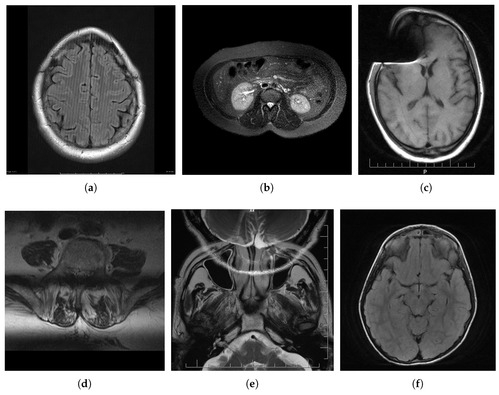
\includegraphics[width=0.78\textwidth]{imagenes/chapter1/MedicalDistortions}
    \end{center}
    \caption{Ejemplo de distorsiones médicas\footnotemark.}
  \end{figure}
  \end{columns}
  \footcitetext{MoreMedicalDistortion}
\end{frame}

\note{
La dificultad nace de la naturaleza de dichas imágenes, que no permiten el uso 
directo de los modelos IQA habituales. Si no que, necesitan que se adapten metódicamente.
O incluso, habitualmente, la adquisición de 
datos a través de escaneo, segmentación u obtenidos de algoritmos de reconstrucción 
3D proporcionan información geométrica ya en forma de nubes de puntos.
Es decir, no en todos los casos, tendremos acceso a las imágenes de las que parten 
dichas reconstrucciones, como en es el caso del escaneo láser en investigación forense.

A pesar de ello, el número de métodos propuestos para la estimación de calidad 3D 
decrece sustancialmente. Más aún si se trata del ámbito biomédico. 
}

\subsection{Objetivos}
\begin{frame}
  \frametitle{Objetivos}
  \begin{columns}

    \column{0.3\textwidth}
    \vspace{-1cm}
  \begin{enumerate}
    \item Estudio exhaustivo del estado del arte. 
    \item Generación de datos sintéticos.
    \item Validar métodos más prometedores.
  \end{enumerate}

  \column{0.7\textwidth}
  \vspace{-.2cm}
  \begin{figure}
      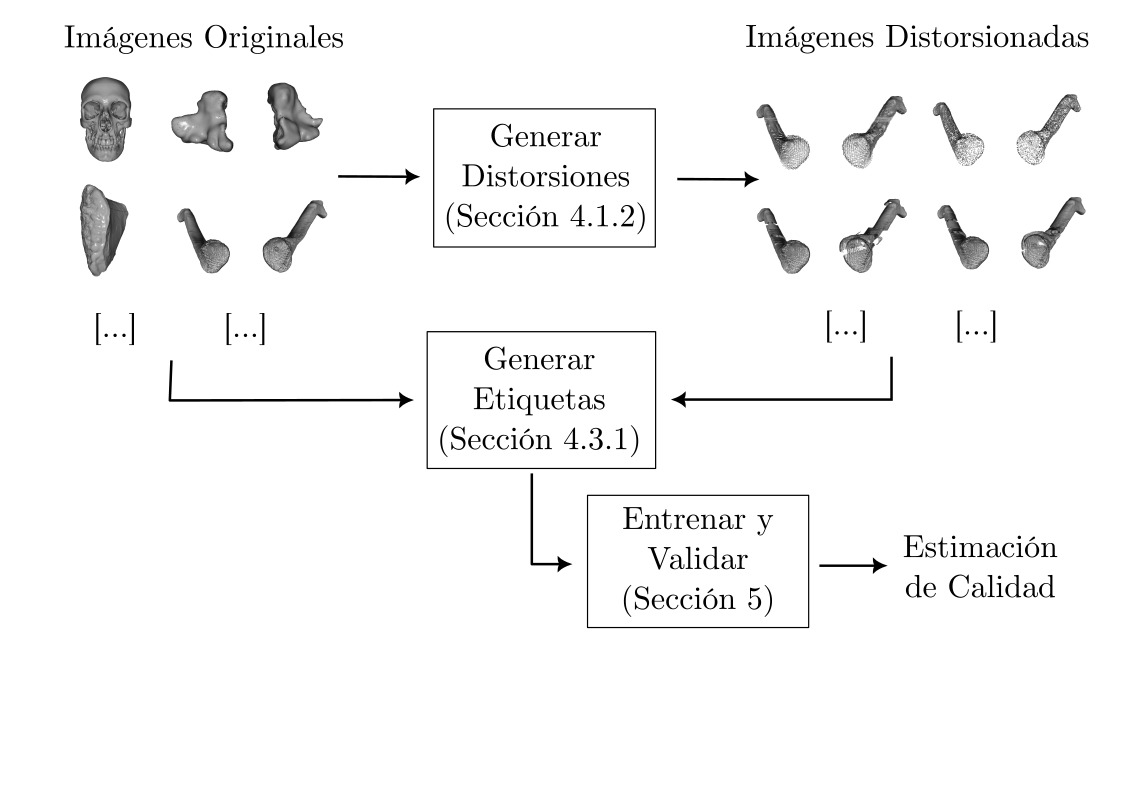
\includegraphics[width=1.0\textwidth, left]{imagenes/chapter1/Objetivos}
  \end{figure}

  \end{columns}
\end{frame}

\note{
Con todo esto, nuestro objetivo se puede descomponer en una serie de metas parciales: 
\begin{itemize}
\item Realizar una revisión exhaustiva del estado del arte
\item Estudiar los patrones de distorsión que afectan a las imágenes biomédicas 3D.
\item Analizar los enfoques más prometedores. 
\item Y, finalmente, generar un conjunto de datos sintético que permita validar 
    las adaptaciones de dichos métodos. Todo ello por medio de un estudio experimental.
\end{itemize}
Resolvamos la primera meta parcial. 
}
